\documentclass[11pt]{beamer}
\usetheme{Warsaw}
\usefonttheme{serif}

\newcommand*\oldmacro{}%
\let\oldmacro\insertshorttitle%
\renewcommand*\insertshorttitle{%
  \oldmacro\hfill%
  \insertframenumber\,/\,\inserttotalframenumber}

\let\olditem=\item% 
\renewcommand{\item}{\olditem \justifying}%


\usepackage{makecell}
\usepackage[utf8]{inputenc}
\usepackage[T1]{fontenc}
\usepackage[french]{babel}
%\usepackage[english]{babel}
\usepackage{ragged2e}
\usepackage{graphicx}
\usepackage{caption}
\usepackage{subcaption}
\usepackage{xcolor}
\usepackage{tcolorbox}
\usepackage{float}
\usepackage{booktabs}
\usepackage{multirow}
\usepackage{array}
\usepackage{tabularx}
\usepackage{graphicx}
\usepackage{longtable}
\justifying
% Setup
\graphicspath{{img/}}
\logo{
\includegraphics[height=5mm]{img/logouniv.png}}

% Metadata
\title{Représentation des connaissances spatiales et modélisation de l'apprentissage des agents pour la simulation de l'utilisation de la terre}
\subtitle{}

%%%%%%%%%%%%%%%%%%%%%%%%%%%%%%%%%%%%%%%%%%%%%%%%%%%%%%%%%%%%%%%%%%%%
\begin{document}
    
  %-------------------------------->
  \begin{frame}[plain]
    % Header
    \begin{figure}
      \vspace{-0.5cm}
      \centering      
      
\includegraphics[width=.8\textwidth]{univ-header.png}
    \end{figure}
    \vspace{-1.2cm}

    % Title
    \author{}
    \date{}
    \titlepage
    \vspace{-2.5cm}
    
    % Authoring
    \centering
    {
      \scriptsize
      
      Par\\[1mm]
      {\bfseries NGOMSEM Ngueramadji}\\[1mm]
      CM-UDS-23SCI0912\\[3mm]
      
      Sous la direction de\\[1mm]
      {\bfseries Dr FOTSING Eric}\\[1mm]
      {\itshape Chargé de cour, Université de Dschang/IUT}\\[3mm]
      
      {\normalsize {\today}} 
    }    
  \end{frame}

  %--------------------------------------------------------
  % Metadata
  \author{NGOMSEM Ngueramadji}
  %--------------------------------------------------------
  
  %-------------------------------->

  %-------------------------------->
  \begin{frame}
\frametitle{Plan de présentation}
\tableofcontents[hideallsubsections]
\end{frame}
  
  \section{Introduction}
  \frame{\tableofcontents[currentsection,hideallsubsections]}
  
  %%
  \subsection{Contexte}
  \begin{frame}
  	% \frametitle{Contexte}
    \begin{figure}
        \centering
        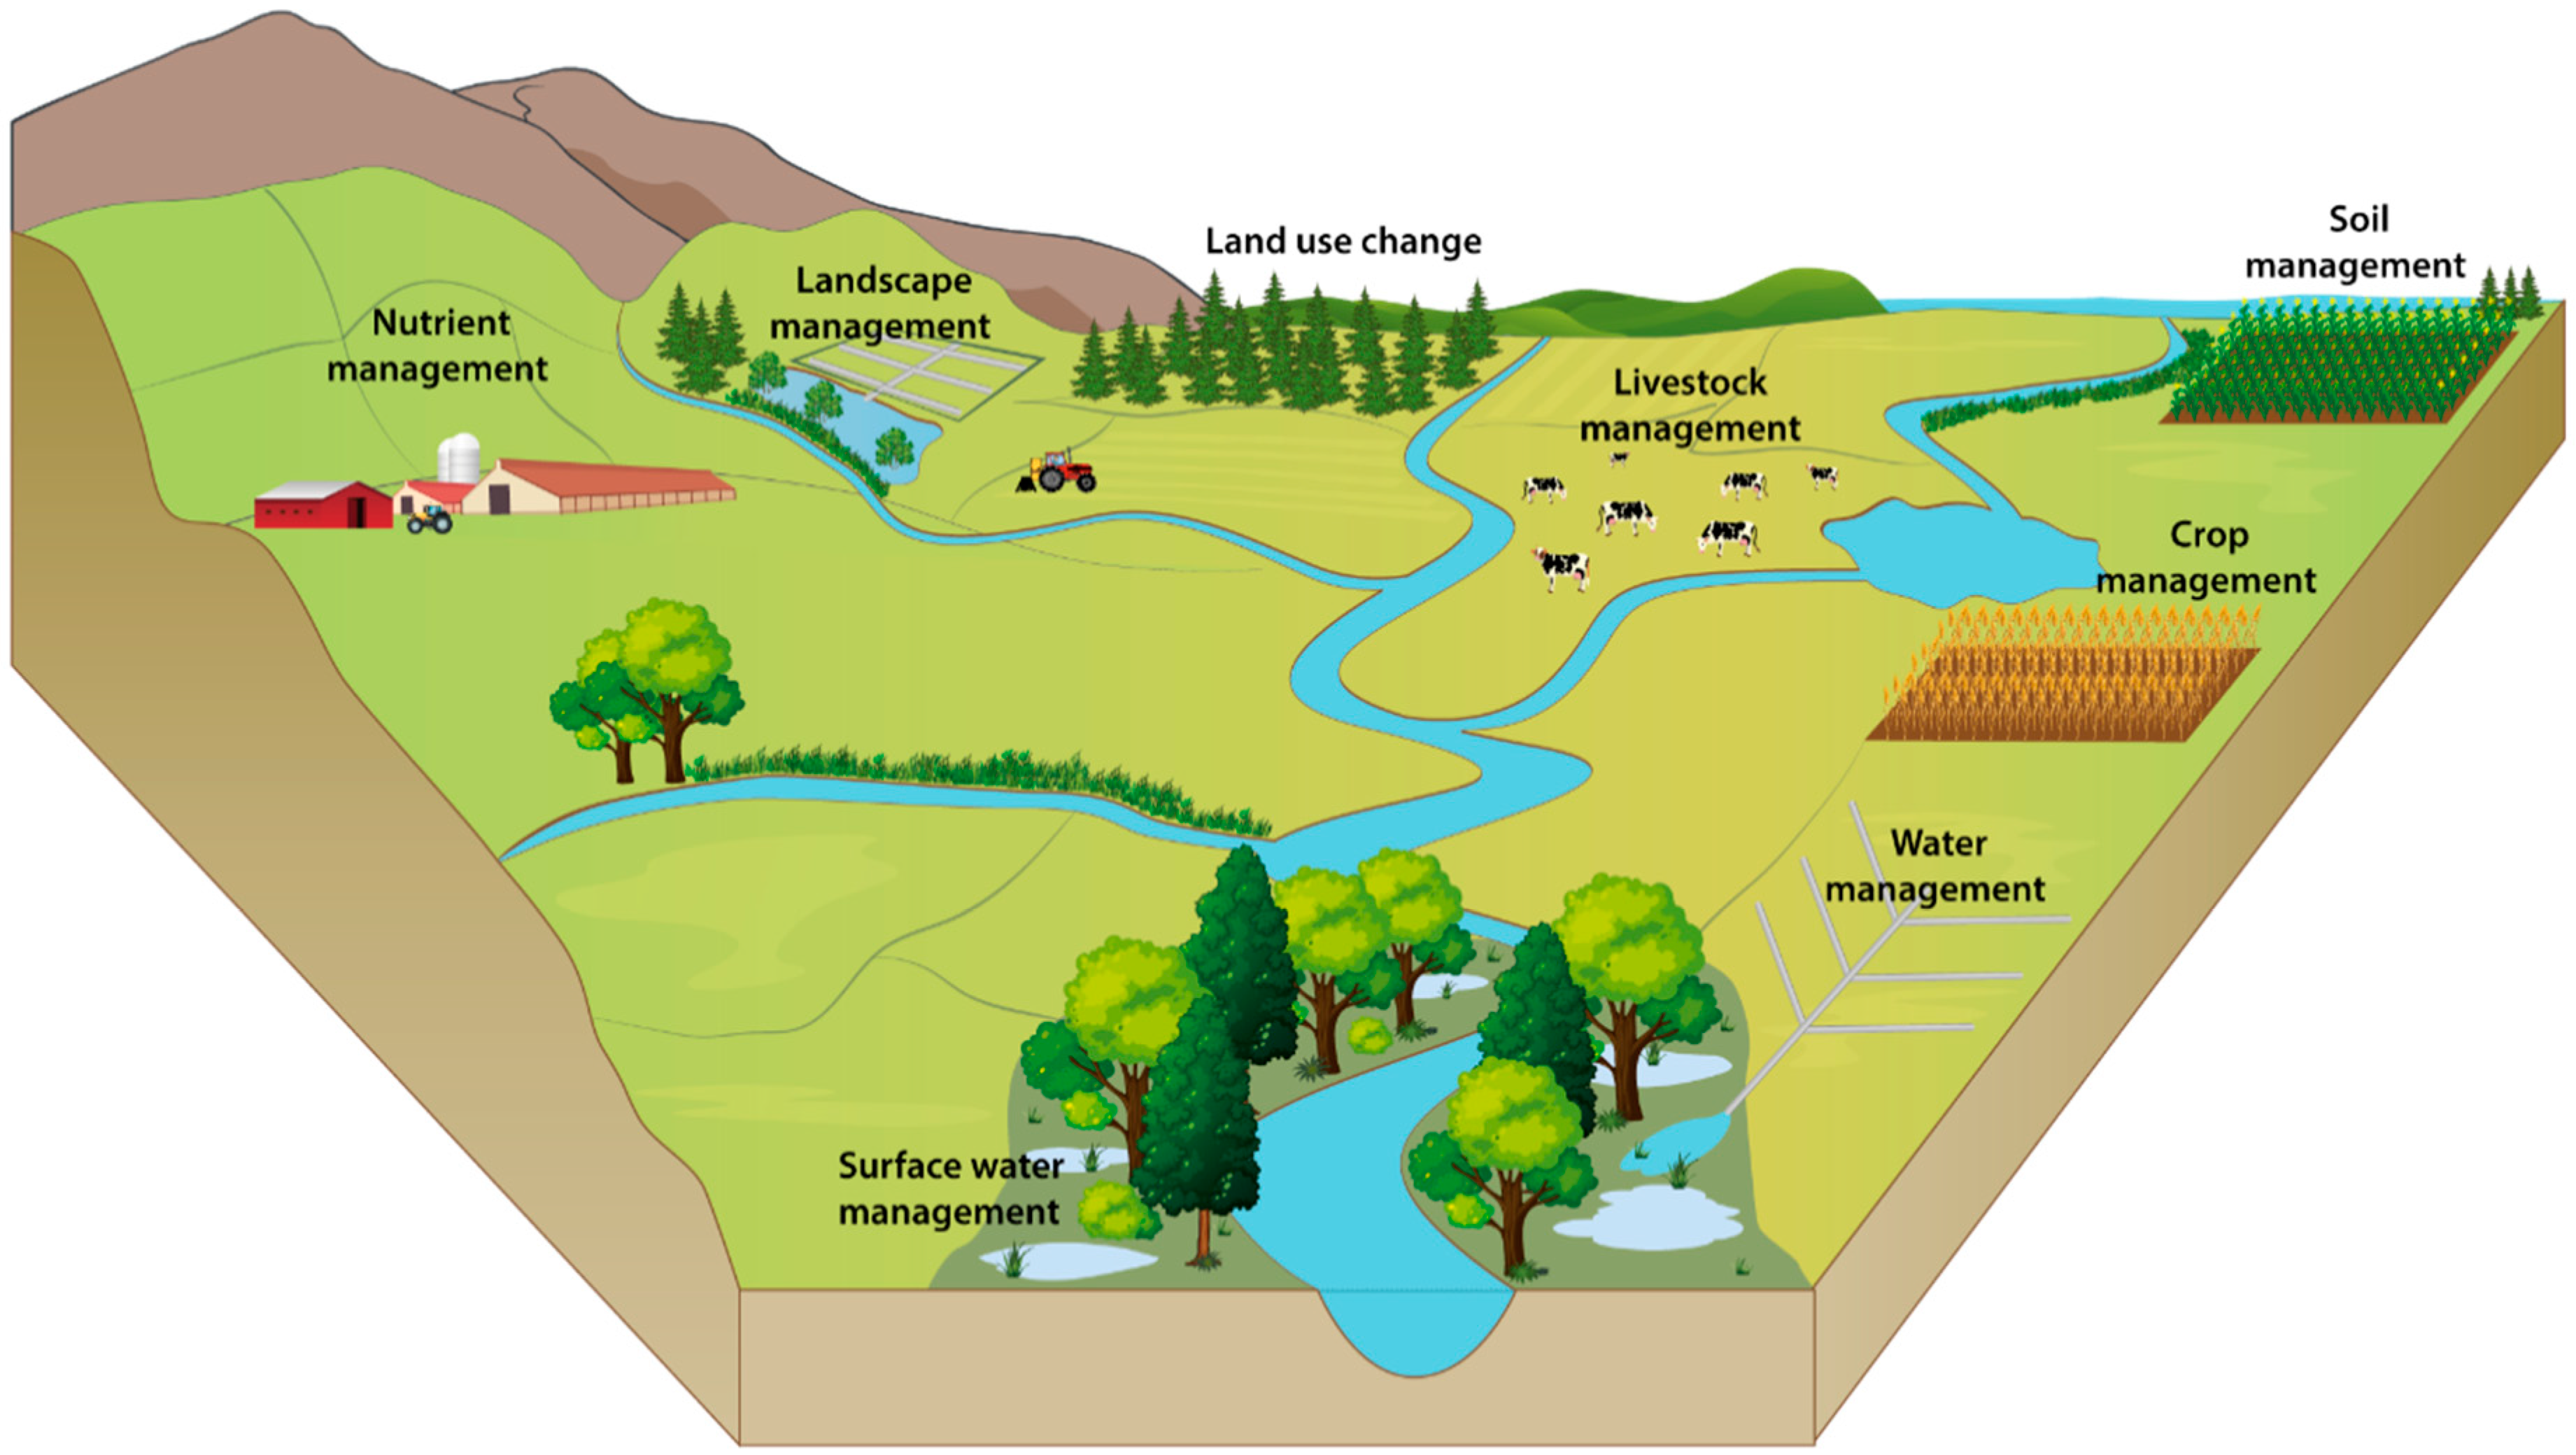
\includegraphics[width=0.9\linewidth, , height=0.8\textheight]{Mes_images/water-12-02412-g001.png}
    \end{figure}
  \end{frame} 

  \begin{frame}
  	% \frametitle{Contexte}
\begin{figure}
    \centering
    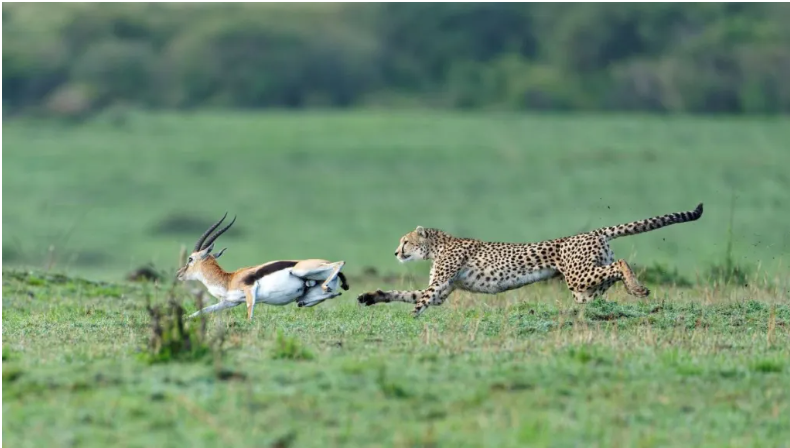
\includegraphics[width=1\linewidth]{Mes_images/prey-predator.PNG}
\end{figure}
  \end{frame}
\begin{frame}
\frametitle{Contexte}
 La chasse dans les écosystèmes implique des interactions
complexes entre prédateurs, proies et ressources (eau,
végétation). Les modèles actuels manquent de
représentations sémantiques et de généralisation pour
capturer ces dynamiques.

\end{frame} 
% \subsection{Contexte général}

% \subsection{Problème et problématique}
\begin{frame}
    \frametitle{Problématique}
    
    \begin{block}{Problématique}
        Comment modéliser un système multi-agent combinant ontologie et apprentissage adaptatif pour simuler la chasse de manière réaliste ?
    \end{block}
 
\end{frame}
\subsection{Objectifs du mémoire}
\begin{frame}
    \frametitle{Objectifs du mémoire}
   \begin{block}{Objectif général}
    L’ambition majeure de cette recherche est la conception et l’implémentation d’un modèle multi agent, basé sur la simulation de la chasse.
   \end{block}
    \begin{block}{Objectifs spécifiques}
    \begin{itemize}
        \item Modéliser les entités de la chasse sous forme d’agents autonomes ;
        \item Concevoir une ontologie de la chasse pour structurer les connaissances utiles à la
             prise de décision ;
        \item Implémenter des mécanismes d’apprentissage pour permettre aux agents d’adapter
            leur stratégie ;
    \end{itemize}
    \end{block}
\end{frame}
\subsection{Méthodologie}
\begin{frame}
\frametitle{Méthodologie}
\begin{block}{Les méthodes}
    \begin{itemize}
    \item Analyse des travaux existants

    \item Conception d’une ontologie de la chasse

    \item Intégration de l’apprentissage Q-learning

    \item Implémentation dans GAMA

    \item Expérimentation et analyse des résultats 
   
    \end{itemize}
\end{block}
\end{frame}

\section{État de l'art}
\subsection{Quelques travaux récents effectués}
\begin{frame}
    \frametitle{Quelques travaux récents effectués}
    \begin{itemize}
        \item Predicting Ecosystem Resilience (2025): Utilise le MARL (Multi-Agent Reinforcement Learning) pour modéliser les interactions proie-prédateur dans un environnement alpin\\
Données réelles intégrées, mais  absence d’ontologie, limitant la structuration sémantique de l’espace.

\item Collaborative Hunting (2024): Repose sur le Deep RL pour simuler la chasse en groupe entre agents.
Modèle collaboratif, mais  ne prend pas en compte les ressources spatiales (eau, herbe), ce qui limite le réalisme écologique.
\end{itemize}
\end{frame}
\begin{frame}
\frametitle{Quelques travaux récents effectués}
 \begin{itemize}
     \item Agent-Based Modeling (2022):
Utilise des règles statiques dans un modèle multi-agent classique, avec données empiriques.
Faible capacité d’adaptation des agents ; pas d’apprentissage.
Valide expérimentalement des dynamiques territoriales.
\item   Survey on Reinforcement Learning (2024):
 Étude théorique des approches d’apprentissage par renforcement.
 Elle ne propose pas de modèle concret, ni d’application à un cas particulier comme la chasse.

 \end{itemize}   
\end{frame}

\subsection{Lacunes identifiées dans les travaux existants}
\begin{frame}
\frametitle{ Lacunes identifiées dans les travaux existants}
\begin{block}{Lacunes identifiés}
\begin{itemize}
    \item Absence de structuration sémantique des connaissances;
    \item Complexité computationnelle excessive;
    \item Manque d’apprentissage adaptatif;
    \item Manque d’intégration des ressources 
\end{itemize}
\end{block}
\end{frame}
\subsection{Positionnement de l’approche proposée}
\begin{frame}
\frametitle{Positionnement de l’approche proposée}
\begin{block}{Approche proposée}
    \begin{itemize}
        \item Ontologie pour la représentation sémantique
        \item Q-learning pour l’efficacité
        \item Généralisation 
        \item Approche hybride(ontologie, apprentissage).
    \end{itemize}
\end{block}
    
\end{frame}
\section{Fondements théoriques et concepts clés}

\subsection{Quelques définitions des concepts clés}
\begin{frame}
\frametitle{Quelques définitions des concepts clés}
\begin{block}{Systèmes multi-agents}
    Un système multi-agents (SMA) représente un groupe d’agents positionnés dans un
environnement spécifique et interagissant selon une structure définie .
\end{block}
\end{frame}
\subsection{Représentation des connaissances (ontologie)}
\begin{frame}
\frametitle{Représentation des connaissances (ontologie)}
\begin{block}{Ontologie}
\textit{ Une ontologie constitue une description claire d’une conceptualisation}   
\end{block}  
\end{frame}
\begin{frame}
    \frametitle{Q-learning et apprentissage par renforcement}
    \begin{block}{Définitions}
        L’apprentissage par renforcement est une méthodologie qui permet à un agent autonome (tel qu’un robot, un agent de dialogue, un personnage dans un jeu vidéo, entre autres) d’apprendre les actions appropriées à entreprendre sur la base d’expériences antérieures, dans le but d’optimiser une récompense mesurable au fil du temps.   
    \end{block}
\end{frame}
\subsection{Simulation multi-agent}
\begin{frame}
\frametitle{}
 \begin{block}{SMA}
     Une simulation multi-agent consiste à modéliser un système à partir d'agents autonomes dotés de comportements individuels, capables de percevoir leur environnement, d’interagir avec d’autres agents, de prendre des décisions et d’apprendre.
 \end{block}   
\end{frame}

\section{Contribution}
    \subsection{Architecture du système}
    \begin{frame}
    \frametitle{Architecture générale du système}
      \begin{figure}
        \centering
        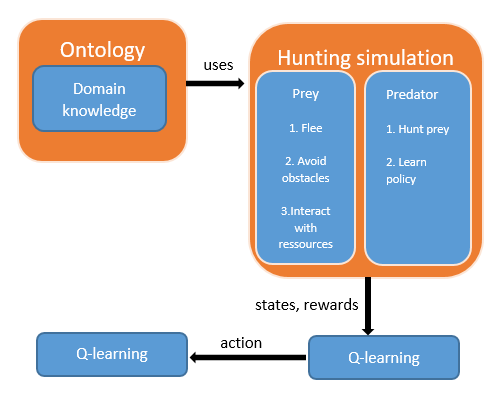
\includegraphics[width=0.9\linewidth, , height=0.8\textheight]{Mes_images/Architecture.PNG}
    \end{figure}  
    \end{frame}
    
    % \subsection{Intégration du Q-learning}
    
\subsection{ Expérimentation}
\subsubsection{Outils utilisés}
\begin{frame}
\frametitle{Outils utilisés et langages}
\begin{block}{Outils}
\begin{itemize}
    \item GIS Agent Based Modeling Architecture, plateforme de modélisation multi-agent;
    \item Protrégé.
\end{itemize} 

\end{block}    
\begin{block}{Langages}
\begin{itemize}
    \item Java;
    \item OWL2;
\end{itemize}   
\end{block}

\end{frame}
\begin{frame}
 \frametitle{Outils utilisés et langage} 
 \begin{block}{Matériels}
PC HP Elitebook pro avec les caratéristiques: 
    \begin{itemize}
    \item 1T SSD;
    \item 16RAM;
    \item Corei7.    
\end{itemize}
    
\end{block}
\end{frame}
% \subsection{Interface de simulation}
\subsubsection{Ontologie construite}
    \begin{frame}
    \frametitle{Ontologie construite}
    \begin{figure}
        \centering
    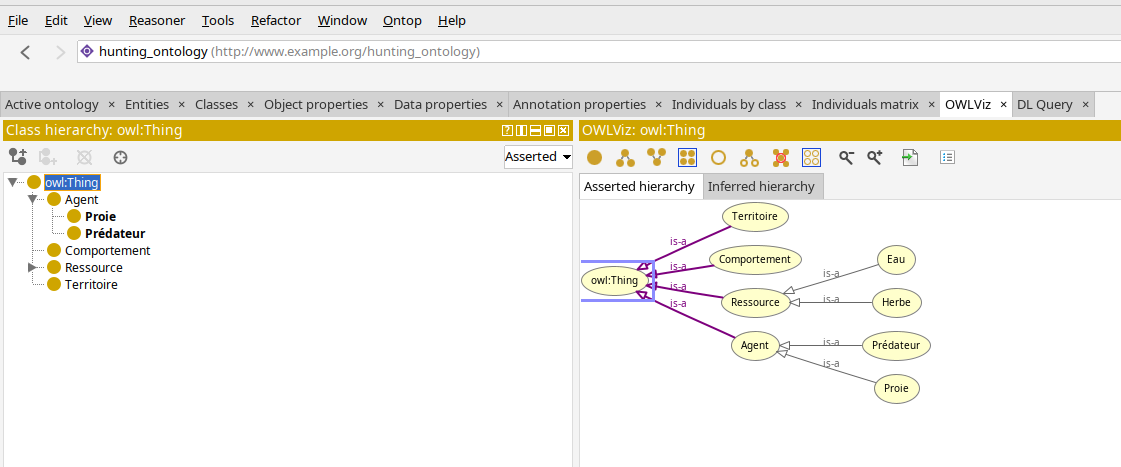
\includegraphics[width=0.9\linewidth, , height=0.8\textheight]{Mes_images/Ontologie créée sous protégé.png}
    \end{figure} 
        
    \end{frame}
\subsubsection{Interface de la simulation}
\begin{frame}
\frametitle{Interface de la simulation}
 \begin{figure}
        \centering
        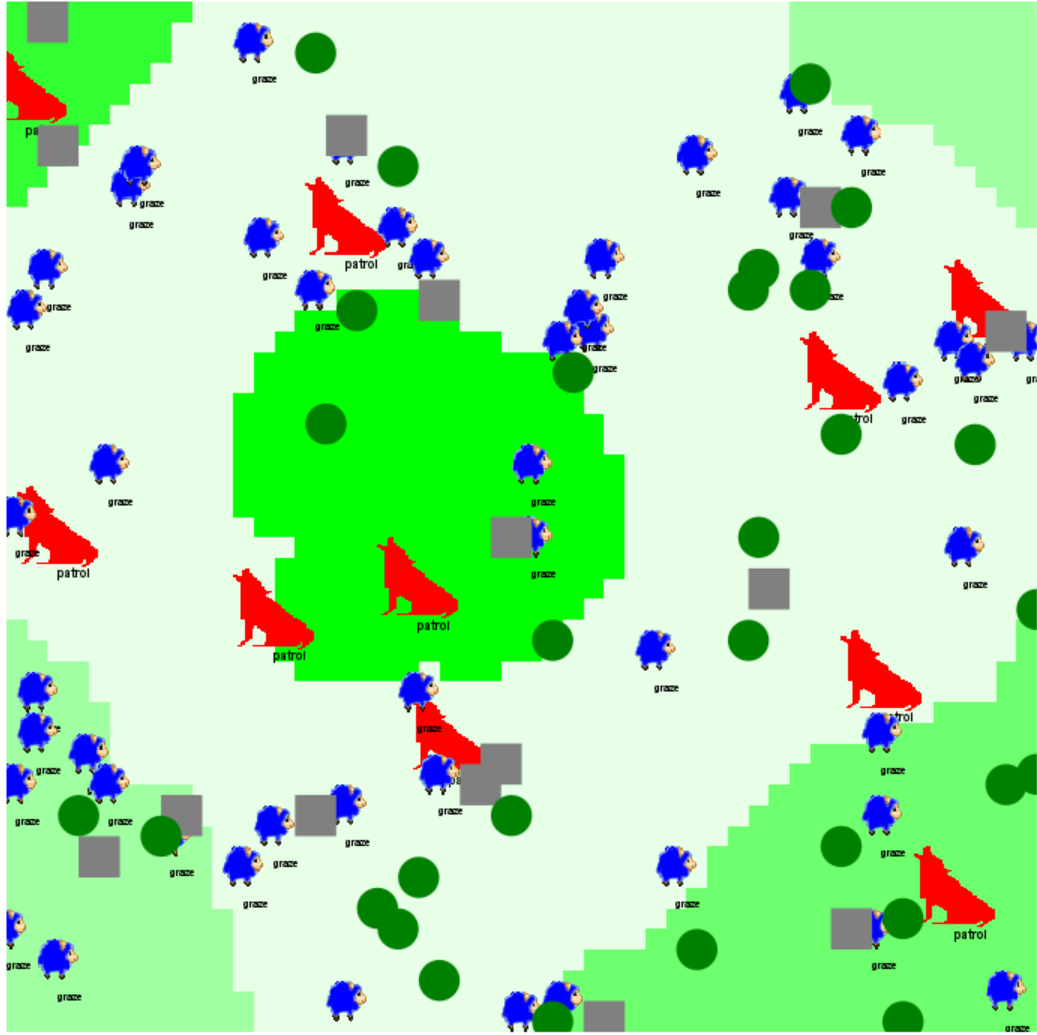
\includegraphics[width=0.9\linewidth, , height=0.8\textheight]{mes_resultats/Interface de simulation.png}
    \end{figure}   
\end{frame}

\subsection{Résultats}
\subsubsection{Évolution des populations}
\begin{frame}
\frametitle{Évolution des populations}
   \begin{figure}
        \centering
        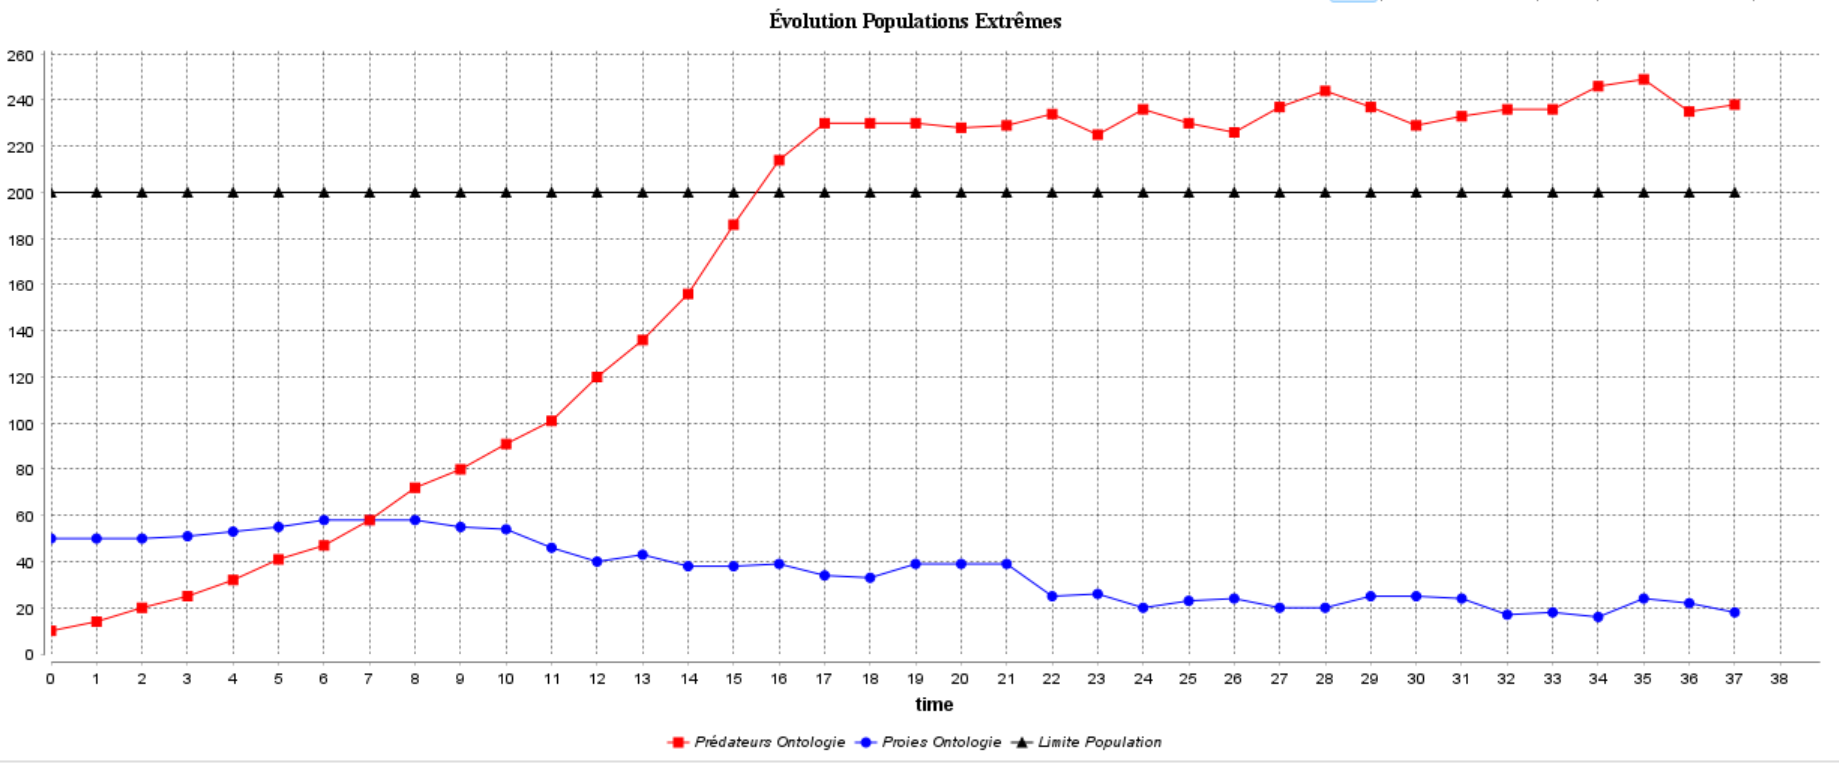
\includegraphics[width=0.9\linewidth, , height=0.8\textheight]{mes_resultats/Evolution des populations.png}
    \end{figure}    
\end{frame}
\subsubsection{Energie moyenne par type}
\begin{frame}
\frametitle{Energie moyenne par type}
   \begin{figure}
        \centering
        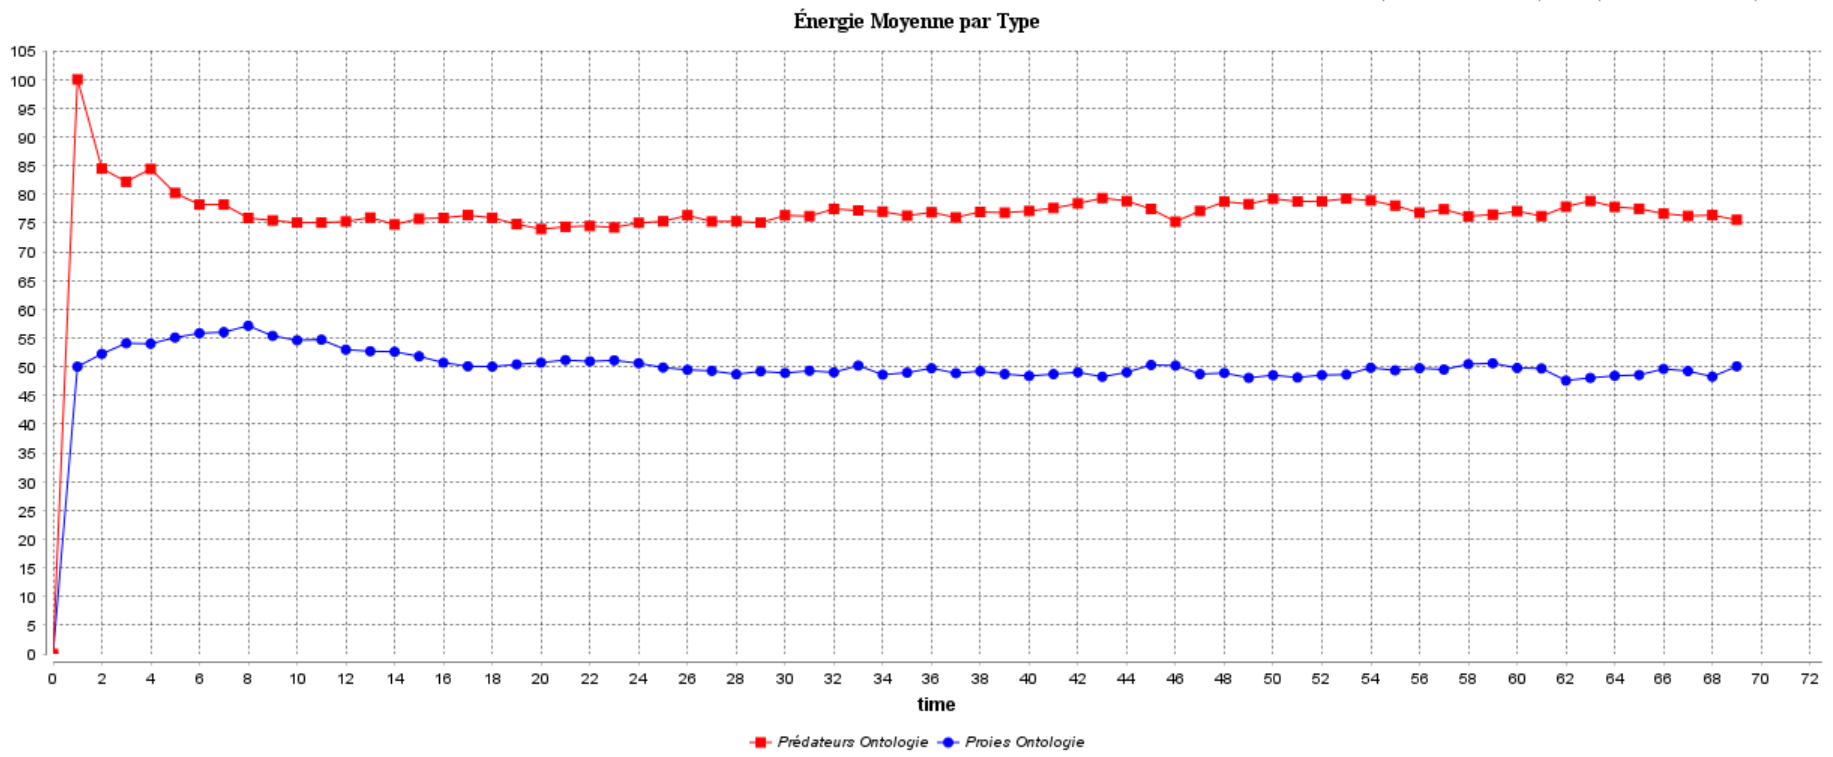
\includegraphics[width=0.9\linewidth, , height=0.8\textheight]{mes_resultats/Energie moyenne par type.png}
    \end{figure}    
\end{frame}
\subsubsection{Naissances cumulées}
\begin{frame}
\frametitle{Naissances cumulées}
   \begin{figure}
        \centering
        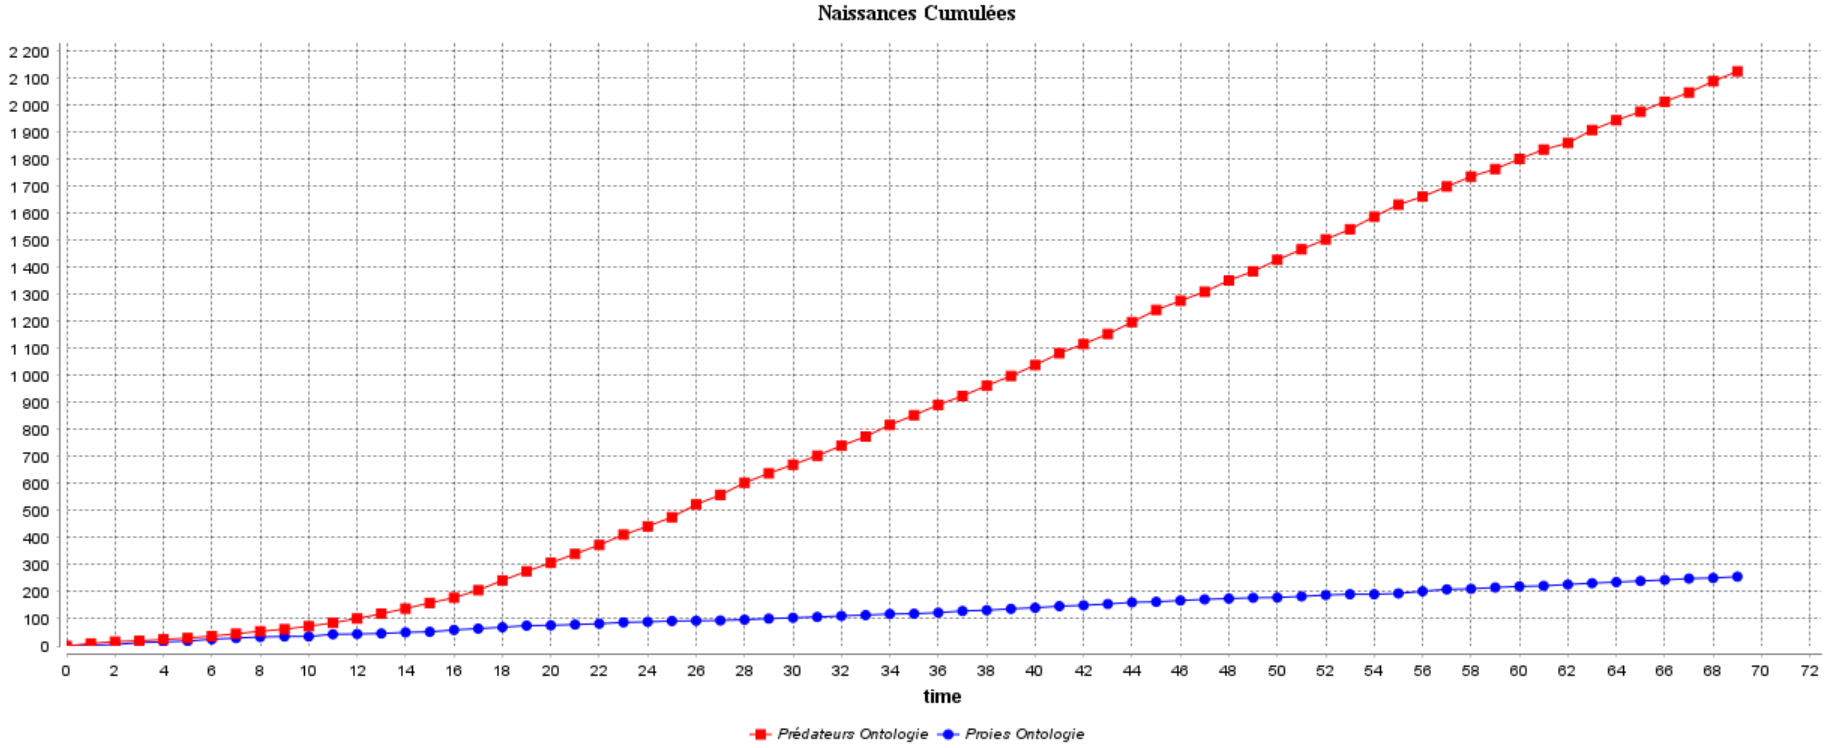
\includegraphics[width=0.9\linewidth, , height=0.8\textheight]{mes_resultats/Naissances cumulées.png}
    \end{figure} 

\end{frame}
\subsubsection{Taux de succès}
\begin{frame}
\frametitle{Taux de succès}
   \begin{figure}
        \centering
        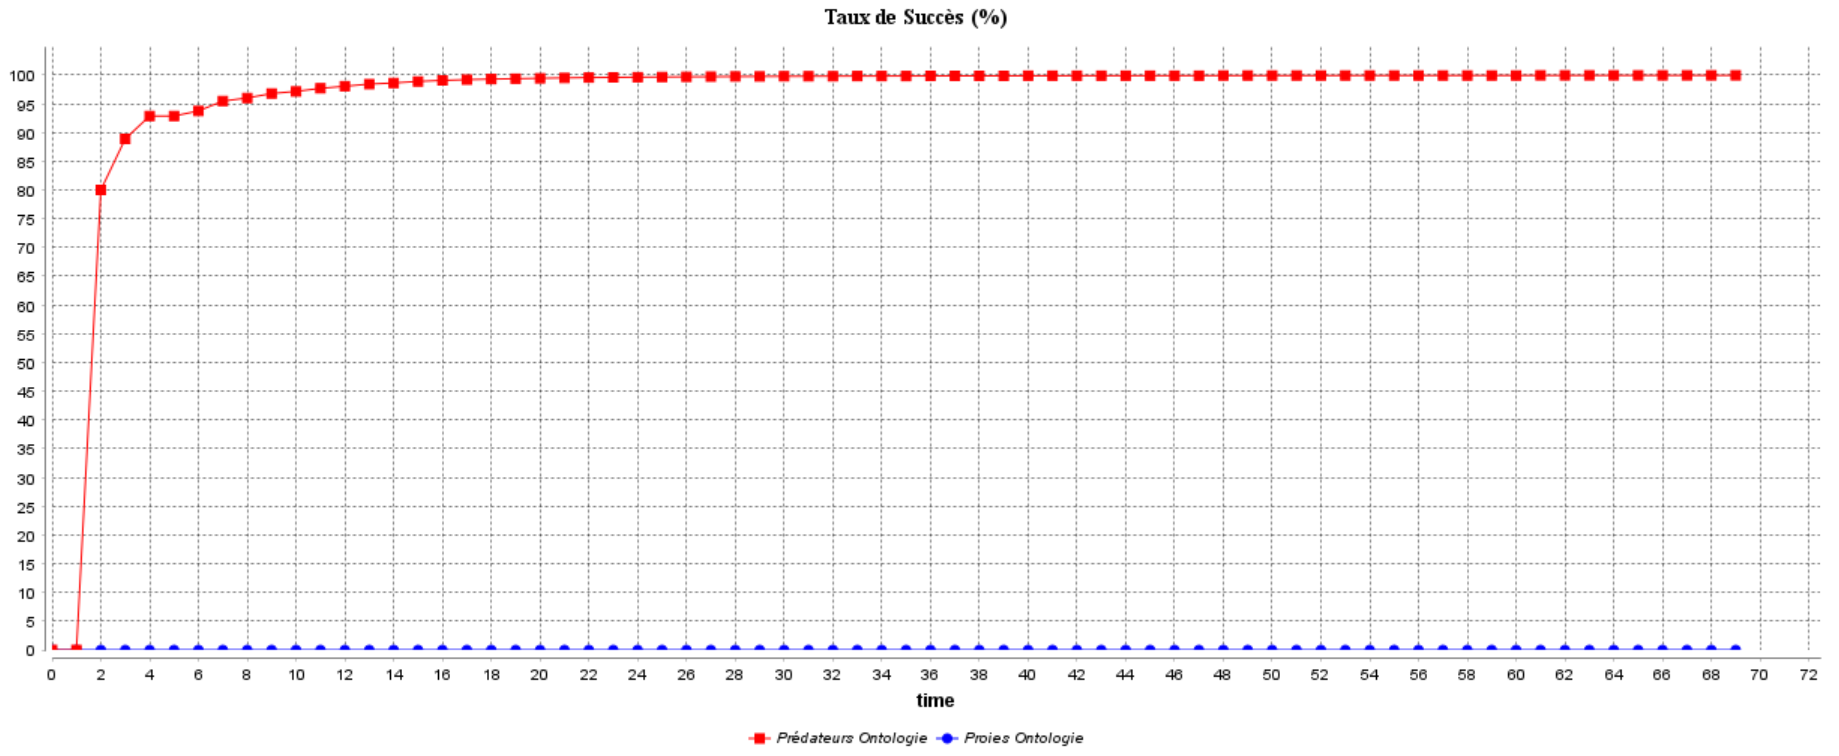
\includegraphics[width=0.9\linewidth, , height=0.8\textheight]{mes_resultats/Taux de succès.png}
    \end{figure}    
\end{frame}
\subsection{Discussion}
% \subsection{Discussion}
\begin{frame}
\frametitle{Discussion}
 \begin{figure}
        \centering
    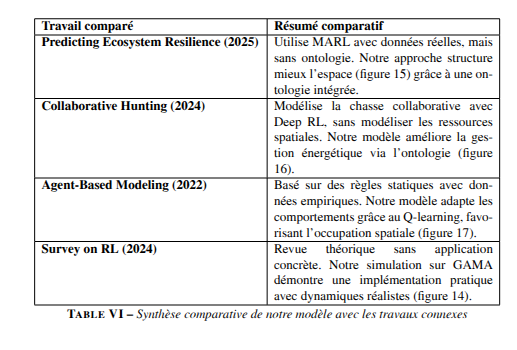
\includegraphics[width=0.9\linewidth, , height=0.8\textheight]{mes_resultats/Capture d’écran du 2025-07-18 11-09-04.png}
    \end{figure}  
    
\end{frame}


\section{ Conclusion}
\subsection{Bilan}
\begin{frame}
\frametitle{ Bilan}
\begin{itemize}
    \item Ce mémoire a permis de concevoir un modèle multi-agent intelligent pour simuler la chasse, combinant ontologie et Q-learning dans GAMA.
    \item Les résultats valident la capacité des agents à apprendre, à interagir de façon crédible avec l’environnement et à optimiser l’usage de l’espace.
    \item L’intégration sémantique améliore la stabilité des dynamiques émergentes par rapport aux approches classiques.
    \item Des limites subsistent, notamment l’absence de données empiriques et la complexité de l’ontologie en environnement dynamique nous ouvrent la porte pour les perspectives futures. 
\end{itemize}
\end{frame}

 
\subsection{Perspectives}
\begin{frame}
\frametitle{Perspectives}
 \begin{itemize}
    \item Intégration de données empiriques pour une validation plus robuste.
    \item Extension du modèle à d’autres écosystèmes (ex. : zones humides, déserts).
     \item Optimisation des algorithmes pour des simulations à plus grande échelle.
    \item Collaboration avec des écologistes pour des applications pratiques.


 \end{itemize}   
\end{frame}

\begin{frame}
\begin{figure}
        \centering
        
\includegraphics[width=0.9\linewidth, , height=0.8\textheight]{Mes_images/8835522.jpg}
\end{figure} 
    
\end{frame}
\end{document}
%%%%%%%%%%%%%%%%%%%%%%%%%%%%%%%%%%%%%%%%%%%%%%%%%%%%%%%%%%%%%%%%%%%%
 \subsection{Définitions}
%   \begin{frame}

%   \frametitle{Quelques définition de base}
%    \begin{block}{Un modèle à base d'agent}Un système multi-agents (SMA) représente un groupe d’agents positionnés dans un
% environnement spécifique et interagissant selon une structure définie
%    \end{block}

%    \vspace{0.5cm}
%   \begin{block}{Un agent}Un agent est une
% entité qui se distingue par son autonomie, même si cette autonomie est partielle.
%    \end{block}
  	
%   \end{frame}
% \subsection{Méthodes courantes }
%  \begin{frame}
%   \frametitle{Méthodes basées sur les modèle mathématiques} 
%    \begin{block}{Modèle de Lotka-Volterra}Le modèle de Lotka-Volterra est un modèle mathématique classique qui décrit les interactions entre une population de proies (notée \( x(t) \)) et une population de prédateurs (notée \( y(t) \)) à l’aide d’un système d’équations différentielles.
%          \begin{equation}
%             \begin{cases}
%             \frac{dx}{dt} = \alpha x - \beta x y \\
%             \frac{dy}{dt} = \delta x y - \gamma y
%             \end{cases}
%         \end{equation}  
%    \end{block}
%   \end{frame}


%   \begin{frame}
%   \frametitle{Méthodes basées sur les modèle mathématiques}
%  \begin{block}{Modèle de Rosenzweig-MacArthur }Le modèle de Rosenzweig-MacArthur est une extension du modèle de Lotka-Volterra.
% \begin{equation}
% \begin{cases}
% \frac{dx}{dt} = r x \left(1 - \frac{x}{K} \right) - \frac{a x y}{1 + a h x} \\
% \frac{dy}{dt} = e \cdot \frac{a x y}{1 + a h x} - m y
% \end{cases}
% \end{equation} 
% \begin{itemize}
%   \item [$\rightarrow$] \( r \) : taux de croissance intrinsèque des proies,
%   \item [$\rightarrow$] \( K \) : capacité de charge de l’environnement,
%   \item [$\rightarrow$] \( a \) : taux d’attaque du prédateur,
%   \item [$\rightarrow$] \( h \) : temps de manipulation,
%   \item [$\rightarrow$] \( e \) : efficacité de conversion alimentaire,
%   \item [$\rightarrow$] \( m \) : taux de mortalité du prédateur.
% \end{itemize}




%  \end{block}


% \end{frame}

%  \begin{frame}
%   	\frametitle{Méthodes basées sur l'apprentissage  automatique}
%   \begin{figure}
%   	\centering      
%   	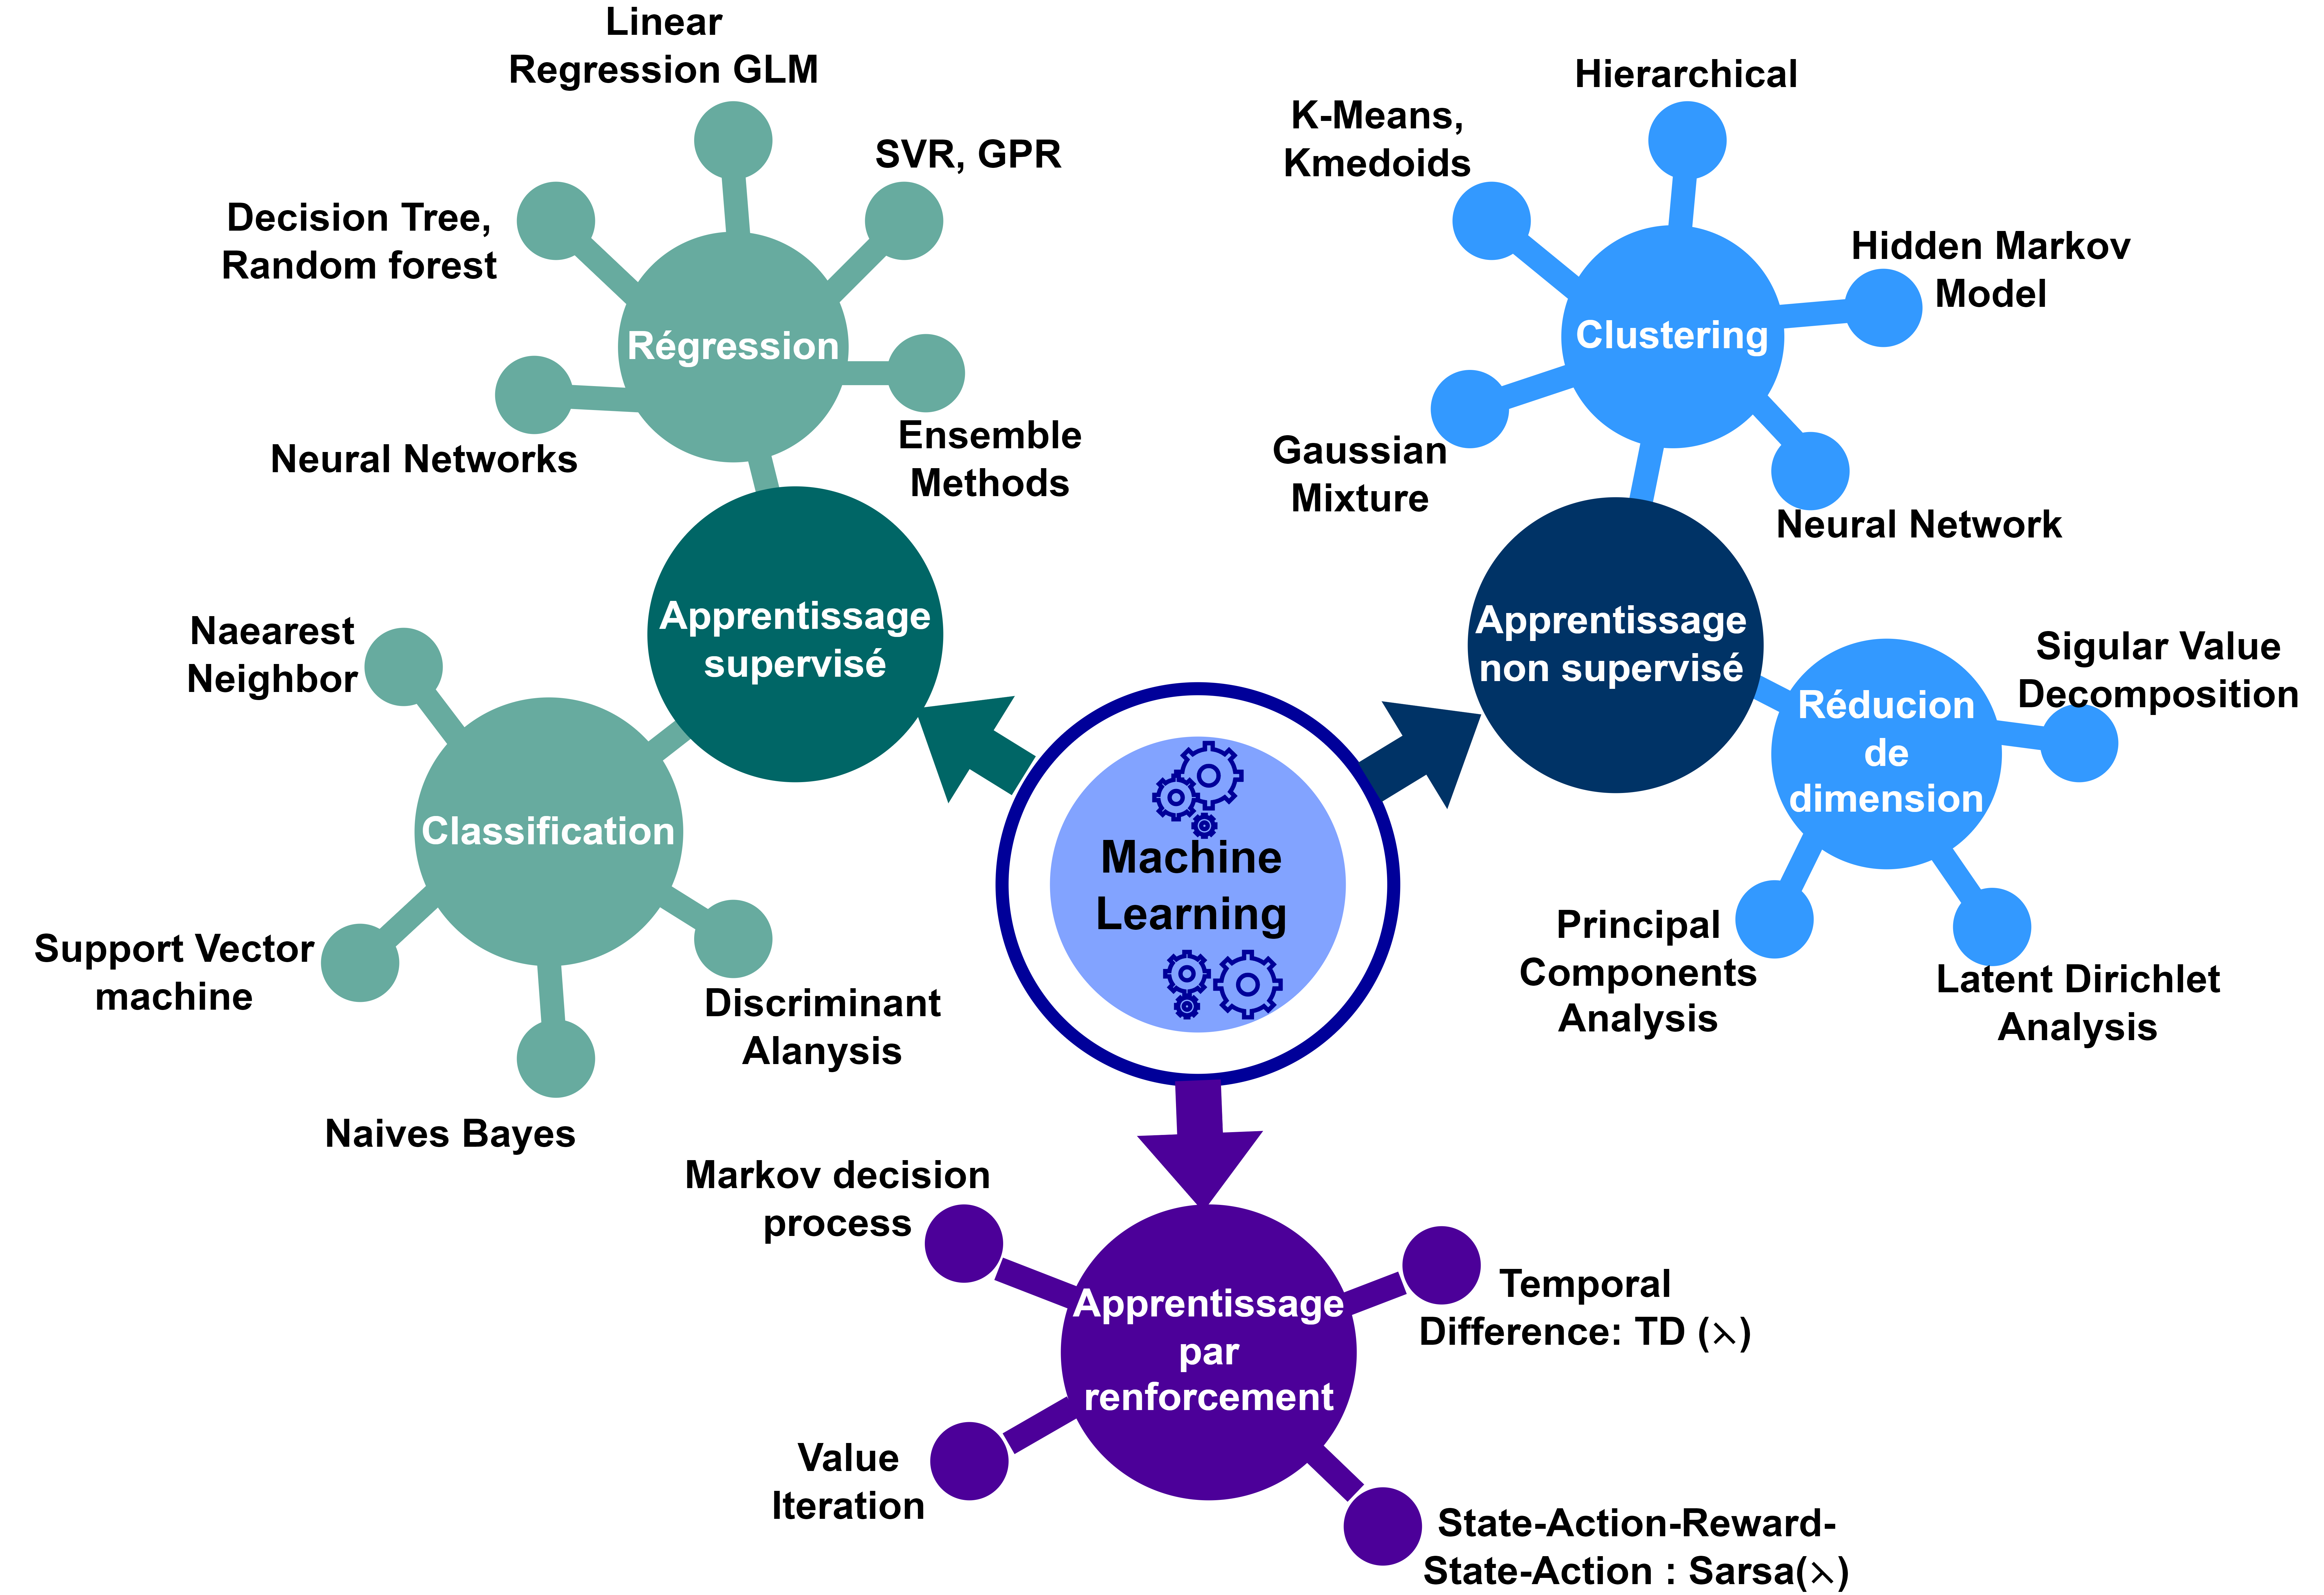
\includegraphics[height=0.75\textheight]{img/ml_alg.png}
%   \end{figure} 
%   \end{frame}  


%   \begin{frame}
%   \frametitle{Méthodes basées sur l'apprentissage  automatique}
%  \begin{block}{Inconvénient } 
%     \begin{itemize}
%         \item  Complexe et difficile à mettre en place.
%     \end{itemize}
%  \end{block}
 
% \vspace{0.7cm}
%  \begin{block}{Avantages}
% \begin{itemize}
% \item Capacité à généraliser sur l'identification des nouveaux gènes et protéines;
% \item Tient compte du contexte de chaque mot avant de pouvoir l'identifier comme un gène ou une protéine.
% \end{itemize}
% \end{block}

% \end{frame}

% \subsection{Motivation}
% \begin{frame}
%     \frametitle{Motivation}
%     \begin{enumerate}
%     \item Améliorer la qualité de prédiction des modèles actuels en réduisant au maximum le nombre de faux positifs et de faux négatifs ;
%     \vspace{0.7cm}
%     \item Exploiter les points forts des modèles de pointe actuels afin d'obtenir de meilleurs résultats.
% \end{enumerate}
% \end{frame}


% \subsection{Problématique étudiée}
% \begin{frame}
%     \frametitle{Problématique étudiée}
%        \begin{block}{Problématique}
%         Comment améliorer les performances de reconnaissance d'entités  nommées de gènes et de protéines en exploitant les performances des modèles existants ?
%        \end{block}
%     \end{frame}

%     \subsection{Objectifs}
%     \begin{frame}
%         \frametitle{Objectif}
%         \begin{block}{Objectif  principal}
%         Proposer une nouvelle architecture de modèle qui offre des performances améliorées par rapport aux modèles de pointe actuels pour la reconnaissance d’entités nommées (REN) de gènes et de protéines.
%        \end{block}
%     \end{frame}

% \begin{frame}
% \frametitle{Objectifs  spécifiques }

%      \begin{itemize}
%             \item Concevoir et implémenter un modèle d’apprentissage automatique qui intègre les points forts de BioBERT et HunFlair; 
            
%             \vspace{0.4cm}
%             \item Harmoniser les disparités dimensionnelles entre les embeddings fournis par BioBERT et ceux attendus par HunFlair;
            
%             \vspace{0.5cm}
%             \item Évaluer et comparer les performances du nouveau modèle par rapport aux modèles existants.
%         \end{itemize}

% \end{frame}
%   %-------------------------------->
%   \section{État de l'art sur les systèmes multi-agents de la chasse }
%   \frame{\tableofcontents[currentsection,hideallsubsections]}

% \subsection{BERT}
% \begin{frame}
% \frametitle{Approche basée sur les Transformers}

% \textbf{Jacob Devlin et al, 2019}.\\
% \vspace{0.4cm}
% Introduisent le modèle\textbf{ BERT} (Bidirectional Encoder Representations from Transformers)
% \vspace{0.3cm}

% \begin{block}{Avantage}
% \begin{itemize}
% \item Efficace en Traitement Automatique du Langage Naturel (TALN).
% \end{itemize}
% \end{block}

% \vspace{0.7cm}
% \begin{block}{Limite}
% \begin{itemize}
% \item Manque de précision dans le cadre biomédical.
% \end{itemize}
% \end{block}
 
% \end{frame}

% \subsection{BioBERT}
% \begin{frame}
% \frametitle{Approche basée sur les Transformers}
% \textbf{Lee et al, 2020}.\\
% \vspace{0.4cm}
% Introduisent le modèle\textbf{ BioBERT} (Biomedical BERT)
% \vspace{0.3cm}

% \begin{block}{Avantage}
% \begin{itemize}
% \item Capte mieux le contexte biomédical des mots.
% \end{itemize}
% \end{block}

% \vspace{0.7cm}
% \begin{block}{Limite}
% \begin{itemize}
% \item Sous-utilise les caractéristiques syntaxiques.
% \end{itemize}
% \end{block}
% \end{frame}

% \subsection{BioByGANs}
% \begin{frame}
% \frametitle{Approche basée sur les Transformers}
% \textbf{Zheng et al, 2022}.\\
% \vspace{0.4cm}
% Introduisent le modèle\textbf{ BioByGANs} 
% \vspace{0.3cm}
% \begin{block}{Avantage}
% \begin{itemize}
% \item Représentation vectorielle des mots nettement plus riche.
% \end{itemize}
% \end{block}

% \vspace{0.7cm}
% \begin{block}{Limite}
% \begin{itemize}
% \item Manque une meilleure précision pour la REN de gènes et de protéines.
% \end{itemize}
% \end{block}
% \end{frame}

% \subsection{HunFlair-Gène}
% \begin{frame}
% \frametitle{Approche basée sur le BiLSTM-CRF}
%   \textbf{Akbik et al, 2022}.\\
% \vspace{0.4cm}
% Introduisent le modèle\textbf{ HunFlair-Gène} 
% \vspace{0.3cm}

% \begin{block}{Avantage}
% \begin{itemize}
% \item Meilleure précision dans l’étiquetage de séquences spécifiques aux gènes et aux protéines.
% \end{itemize}
% \end{block}

% \vspace{0.7cm}
% \begin{block}{Limite}
% \begin{itemize}
% \item L'intégration limitée des contextes larges.
% \end{itemize}
% \end{block}
% \end{frame}

% \subsection{Limites de la Littérature }
% \begin{frame}
%     \frametitle{Limites des Approches d'apprentissage automatique existantes}
%     \begin{enumerate}
%         \item Manque de précision dans l’étiquetage de séquences spécifiques aux gènes et protéines (cas de BERT, BioBERT, BioByGANs) ;
%         \vspace{0.3cm}
%         \item Intégration limitée des contextes larges (cas de HunFlair).
%     \end{enumerate}
% \end{frame}


% \section{Contribution}
% \frame{\tableofcontents[currentsection,hideallsubsections]}

% \subsection{Architecture du modèle proposé}
% \begin{frame}
%     \frametitle{Architecture du modèle proposé}

%     \begin{figure}
%         \centering
%         \includegraphics[width=0.8 \textwidth, height=0.8\textheight]{modèle.drawio (6).png}
%     \end{figure}
% \end{frame}

% \begin{frame}
%     \frametitle{Chargement et prétraitement des données }

%     \begin{figure}
%         \centering
%         \includegraphics[width=1\linewidth]{archi1.png}
%     \end{figure}
% \end{frame}

% \begin{frame}
%     \frametitle{Couche d'embeddings }

%     \begin{figure}
%         \centering
%         \includegraphics[width=1\linewidth]{archi2.png}
%     \end{figure}
% \end{frame}


% \begin{frame}
%     \frametitle{Couche de Reprojection }

%    \begin{figure}
%        \centering
%        \includegraphics[width=1\linewidth]{archi33.png}
%    \end{figure}
% \end{frame}

% \begin{frame}
%     \frametitle{Traitement séquentiel et étiquetage}

%   \begin{figure}
%       \centering
%       \includegraphics[width=1\linewidth]{archi4.png}
%   \end{figure}
% \end{frame}

% \subsection{Environnement de travail}
% \begin{frame}
%     \frametitle{Environnement de travail}
%     Outils utilisés:
%     \begin{enumerate}
%      \item \textbf{Python:} Langage de programmation
%         \vspace{0.5cm}
        
%     \item \textbf{Flair NLP} : Nous avons utilisé la bibliothèque Flair pour ses capacités avancées en traitement du langage naturel, en particulier pour les tâches de REN.
%     \vspace{0.5cm}

%     \item \textbf{Jetstream2 ( 64 Cœurs + 256Go RAM)} : Pour lancer nos entraînements sur des instances, 
%     \end{enumerate}
% \end{frame}

% \subsection{Jeux de données }
% \begin{frame}
% \frametitle{Jeux de données}
%   13 jeux de données ont été utilisés pendant l'entrainement

%    \begin{itemize}
%        \item BC2GM
%        \item BIO INFER
%        \item CELL FINDER
%        \item CHEBI
%        \item DECA
%        \item FSU
%        \item GPRO
%        \item IEPA
%        \item JNLPBA
%        \item LOCTEXT
%        \item MIRNA
%        \item OSIRIS
%        \item VARIOME
%    \end{itemize}
% \end{frame}

% \subsection{Résultats }
% \begin{frame}
%     \frametitle{ Courbes de Perte et de F1-Score}
%     \begin{figure}
%          \centering
%          \includegraphics[width=1\linewidth]{training1.png}

%      \end{figure} 
% \end{frame}


% \begin{frame}
%     \frametitle{Scores }
%    \begin{figure}
%        \centering
%        \includegraphics[width=1\linewidth]{scores-finals.png}
%    \end{figure}
% \end{frame}

% \subsection{Discussions }
% \begin{frame}
%     \frametitle {Discussions sur la précision }
%     \begin{figure}
%         \centering
%         \includegraphics[width=1\linewidth]{precision-final1.png}
%     \end{figure}
% \end{frame}


% \begin{frame}
%     \frametitle{Discussions sur le Rappel}
% \begin{figure}
%     \centering
%     \includegraphics[width=1\linewidth]{rappel-final2.png}
% \end{figure}
% \end{frame}


% \begin{frame}
%     \frametitle{Discussions sur le F1-Score}
% \begin{figure}
%     \centering
%     \includegraphics[width=1\linewidth]{f1-score-final-2.png}
% \end{figure}
% \end{frame}

% \subsection{Test }
% \begin{frame}
%     \frametitle{Résultats}
%    \begin{figure}
%        \centering
%        \includegraphics[width=1\linewidth]{résultats_concret.png}
%    \end{figure}
% \end{frame}

% \section{Conclusion}
% \frame{\tableofcontents[currentsection,hideallsubsections]}

% \subsection{Bilan }
% \begin{frame}
% \frametitle{Bilan}
%    Face à notre problématique, nous avons proposée une nouvelle architecture de modèle qui offre des performances améliorées par rapport aux modèles de pointe actuels pour la REN de gènes et de protéines.
%    \vspace{0.4cm}
   
%     \begin{itemize}
%         \item  Réduire au maximum le nombre de faux positifs et de faux négatifs ;
%         \vspace{0.4cm}
%         \item Exploiter les points forts des modèles de pointe actuels (Biobert et Hunflair).
% \end{itemize}
% \end{frame}

% \subsection{Critiques et Perspectives }
% \begin{frame}
% \frametitle{Critiques et Perspectives}
% \begin{block}{Critiques } 
%     \begin{itemize}
%         \item  Sous utilise les informations syntaxiques;
%         \item Utilise un même label pour les gènes et les protéines. 
%     \end{itemize}
%  \end{block}
 
% \vspace{0.7cm}
%  \begin{block}{perspectives}
% \begin{itemize}
% \item Amélioration des performances de notre modèle en intégrant les informations syntaxiques pour obtenir une représentation vectorielle des mots bien plus riche ;
% \item Consevoir un dataset avec des labels différents pour les gènes et protéines ;
% \item Intégrer le modèle dans des systèmes cliniques.
% \end{itemize}
% \end{block}
% \end{frame}


% \subsection{Code source}
% \begin{frame}
%     \frametitle{Code source}
%    \begin{figure}
%        \centering
%        \includegraphics[width=1\linewidth]{code_source.png}
%    \end{figure}
% \end{frame}

% %-------------------------------->
% \subsection{}
%   \begin{frame}
%     \centering    	
%     \usebeamerfont{frametitle}{\huge{Merci pour votre attention :-$)$}}
%   \end{frame}
